\chapter{Introduction}\label{section:introduction}
\thispagestyle{pagestyle}


\section{CONTEXT}

Agriculture is a vital sector that plays a crucial role in sustaining human life and the economy.
Agriculture automation and optimization has become a major concern in recent years. 
As the global population continues to grow, the demand for food is increasing and the developing need for food
along with the effect of climate changes are forcing the agricultural industry to adapt and innovate\cite{OBAIDEEN2022100124}.

In the last 35 years, the wold has seen a doubling of the agricultural production. This has been achieved throught the use
of different fertilizers, pesticides and herbicides. This doubling was associated with a 6.87-fold increase in nitrogen fertilization,
a 3.48-fold increase in phosphorus fertilization and 1.68-fold increase in the amount of irrigated cropland \cite{doi:10.1073/pnas.96.11.5995}.
In addition, the water consumoption is expected to increase by 50\% by 2050 \cite{s20236865}. 

This project aims to address the challenges of water scarcity and the need of efficient irrigation systems
by presenting the plan, the implementation, the results and future work of a system that can be used in different
scenarios and is meant to help reducing the water consumption and increasing the agricultural productivity.
The PiIrrigate project intends achuive this by developing an innovative irrigation system that leverages the power of 
IoT and LoRa radio communication technologies.  
The main focus of this project is to create a system that can be easly used in different agricultural settings, 
starting from small gardens to large farms and even smart greenhouses. Beside this, I wanted to create a system that 
is easy to use and can be extended with ease. 

The ESP32 boards with sensors are responsible for colecting the data. Then data is sent using  LoRa to another
ESP32 board that acts as a gateway connected to a Raspberry Pi, which is responsible for sending the data to a web API.
The web API is developed in .NET and is responsible for storing the data in a PostgreSQL database.
The data is then sent to a web application using SignalR, which allows real-time communication between the server and the client.
The web application is responsible for displaying the live data and the historical data and also for providing a way to
control the system manually and to add new nodes to the system. 

This system takes advantage of the LoRa radio communication technology, 
which allows for long-range communication with low power consumption. Meaning that the system can be used in remote areas and
it will work even if the internet connection is not available to all the nodes. The Raspberry Pi is the only component of this system
that needs to be connected to the internet. Other components can be scatered on a area of 10km or more, depending on
the environment and the node setup (mesh or star topology).

\newpage
\section{MOTIVATION}


The reason why I choose to create such a system was fulled by my passion for technology and smart agriculture. Besides this,
I like to observe the data path, from the moment it is collected by the sensors, to the moment it is displayed
in a web application. 
I have always been intested in pieces of technology that can be used to solve real world problems and now I had the chance
to create such a system.

Initially, I wanted to create a system for my own lawn, but as I started working on the project, I realized that the system
can be used in many other scenarios, such as smart greenhouses or even large farms or vineyards. 

\chapter{State of the Art}\label{section:stateoftheart}

\section{Introduction}
The state of the art chapter provides an overview of the current state of smart irrigation 
systems and their applications in agriculture. 
This chapter will explore the existing technologies, methods, and solutions used in smart irrigation. 
It will also highlight the gaps and challenges in the current systems,
and how the PiIrrigate project aims to address these issues.

\section{Existing Smart Irrigation Solutions}
\subsection{Types of Smart Irrigation Systems}

There are several types of smart irrigation systems used in modern agriculture:

\begin{itemize}
  \item \textbf{Weather-Based Controllers} \\
  These systems use weather data to adjust irrigation schedules based on evapotranspiration rates, 
  ensuring that plants receive the right amount of water.

  \item \textbf{Soil Moisture-Based Controllers} \\
  These systems rely on data from soil moisture sensors placed in the root zone of the plants.
  Irrigation cycles are triggered when the soil moisture drops below a predetermined threshold, 
  ensuring plants receive water only when necessary.
  This method is very precise for specific zones\cite{smartIrrigationTechnologyControllersAndSensors}.

  \item \textbf{Hybrid Systems} \\
  Many modern systems utilize a hybrid approach, combining data from both
  weather feeds and soil moisture sensors for more accurate and resilient 
  irrigation decisions. Some research also explores "hybrid" in terms of 
  integrating different energy sources (e.g., solar and wind) to power the systems or 
  combining various 
  irrigation methods (like drip and sprinkler) under one smart control\cite{soilBasedIrrigation}.

  The PiIrrigate project place itself in the category of hybrid systems, using both
  soil moisture sensors and weather sensors to collect data.
  
  Some of the most popular hybrid smart irrigation systems include:
  \begin{itemize}
    \item \textbf{Netafim's Precision Irrigation System} \\
    This system cobines data from soil moisture and flow sensors with sattelite weather data and predictive
    analytics to optimize the irrigation proccess.
    
    Key features include:
    \begin{itemize}
      \item Real-time monitoring of soil moisture levels and weather forecasts.
      \item Automated irrigation scheduling based on weather forecasts.
      \item AI-based algorithms to optimize the irrigation timing and duration.
    \end{itemize}

    \item \textbf{CropX Smart Farming System} \\
    CropX is a cloud based platform that integrates soil moisture sensors, weather data and
    machine learning algorithms to optimize the irrigation process.

    Key features include:
    \begin{itemize}
      \item Irrigation recomandations based on soil variability, crop type and weather.
      \item Farmers can apply recommandations or integrate with automated irrigaitons contrllers.
      \item Easy to scale and adapt to different farm sizes from small to large-scale farms.
    \end{itemize}
  
    \item \textbf{Toro EVOLUTION® Series Controller with Smart ET Sensor} \\
    Combines basic sprinkler system hardware with smart sensors and connectivity,
    offering both manual and intelligent irrigation options. The evaporation sensors are used to measure
    the amount of water lost throught evaporation and adjust the irrigation accordingly.

    Key features include:
    \begin{itemize}
      \item Can be programmed manually or connected to a local weather station.
      \item Smart ET sensor measures evaporation rates and adjusts irrigation schedules.
      \item Compatible with smart devices for remote monitoring
    \end{itemize}
  \end{itemize}
\end{itemize}

\section{Comparative Analysis of Smart Irrigation Systems}
The table below provides a comparative analysis of some of the most popular smart 
irrigation systems available today and the PiIrrigate system.

\begin{table}[ht]
\centering
\begin{tabular}{|p{3.2cm}|p{3.2cm}|p{3.2cm}|p{3.2cm}|p{3.2cm}|}
\hline
\textbf{Feature} & \textbf{Netafim} & \textbf{CropX} & \textbf{Toro ET} & \textbf{PiIrrigate} \\
\hline
Irrigation Type & Drip & Any & Sprinkler & Custom \\
\hline
Automation & High (AI) & Med–High & Medium & Medium \\
\hline
Sensors & Soil, flow, weather & Soil, temp & ET sensor & Soil, temp, rain \\
\hline
Weather Data & Yes & Yes & Yes & Optional \\
\hline
Manual Control & App/cloud & App/web & Panel/app & Web UI \\
\hline
AI/Analytics & Yes & Yes & No & No \\
\hline
Scalability & Large farms & Small–large & Residential & Small farms/gardens \\
\hline
Cloud Sync & Yes & Yes & Optional & Yes \\
\hline
Use Case & Precision agri & Smart farming & Lawn care & Small to large scale\\
\hline
Cost & High & Med–High & Low–Mid & Low \\
\hline
\end{tabular}
\caption{Comparison of Smart Irrigation Systems}
\label{tab:irrigation_comparison}
\end{table}

\section{Identified Gaps and Challenges}
Despite the advancements in smart irrigation systems, several gaps and challenges remain:

\begin{itemize}
  \item \textbf{High Costs} \\
  Many existing systems are expensive, making them inaccessible for small farmers or home gardeners.
  
  \item \textbf{Complexity of Use} \\
  Some systems require specialized knowledge to set up and maintain, which can be a barrier for adoption.

  \item \textbf{Limited Customization} \\
  Many systems are designed for specific crops or environments, limiting their applicability in diverse agricultural settings.

  \item \textbf{Data Integration Issues} \\
  Integrating data from multiple sources (e.g., weather, soil sensors) can be challenging, leading to inefficiencies in irrigation management.
\end{itemize}

Bedside the presented gaps, there are also some other challenges that need to be addressed, such as:
data security and privacy concerns, the need for reliable internet connectivity in remote areas, 
and the need for systems that can operate in harsh environmental conditions. 

Another aspect that needs to be considered is the environmental impact of smart irrigation systems.
While these systems are designed to optimize water usage,
the production and disposal of electronic components can have a negative impact on the environment.
So another challenge is to create systems that are environmentally friendly and sustainable. This means 
that the components used in these systems shlould be madea from recyclable materials 
and the systems should be designed to have a long lifespan and to be easily repairable.

\section{Summary}
In summary, the state of the art in smart irrigation systems shows significant 
advancements in technology and methods, but also highlights several gaps and challenges 
that need to be addressed. The PiIrrigate project aims to fill these gaps by providing a
cost-effective, easy-to-use, and customizable solution that leverages the power of IoT and LoRa 
radio communication technologies. 

\chapter{Used Technologies}
\section{Development Process Tools}
\subsection{Version Control: GitHub}
GitHub is a web-based platform that uses Git for version control and collaboration on software projects.
It enables developers to collaborate in real-time. Thhey can track changes, manage issues, and review code.
It was released in 2008 and in 2018 it was acquired by Microsoft\cite{githubDefinition}.
Github is widely used in the software development industry and in has become standard practice to 
use GitHub for version control. 

\subsection{Software Development: Visual Studio Code and Visual Studio}
Visual Studio Code (VS Code) is a free lightweight code editor developed by Microsoft.
It supports a wide range of programming langueges and has a rich collection of extensiont that can be used to 
enchance its functionality.
It was very convinient to use a single code editor for multiple programming languages and frameworks.
To be more specific, I used Visual Studio Code for ESP32 programming, along with Platform IO, 
which is an open-source ecosystem for IoT development. VSCode was also used for the Angular web application 
development. The Raspberry Pi was programmed using Python, I used Visual Studio Code and for remote access
I used SSH.

Visual Studio is a more comprehensive integrated development environment (IDE) that provides advance features
for software development, such as debugging, profiling, and testing.
Visual Studio is also developed by Microsoft and it is widely used in the software development industry.
Since the PiIrrigate's web API was developed in .NET, I used Visual Studio for the API development.

\subsection{System Architecture: Draw.io}
Draw.io is a free online diagramming tool that allows users to create flowcharts, 
UML diagrams, network diagrams, and more. 
Other alternatives include Lucidchart, Microsoft Visio, and Gliffy. But I found that Draw.io is easy to use
and provides a wide range of templates and shapes that can be used to create diagrams.

\subsection{Iot Device Management: Azure IoT Hub}
Azure IoT Hub is a cloud-based service that enables secure and reliable 
communication between IoT devices and the cloud.
It provides a way to connect, monitor, and manage IoT devices at scale.
Azure IoT Hub is used in the PiIrrigate project to manage the
communication between the Raspberry Pi and the web API.

\section{Communication Technologies}
\subsection{LoRa Radio Communication}
LoRa is a wireless modulation technique derived from Chirp Spread Spectrum (CSS) technology.
LoRa modulated transmission is robust against disturbances and can be received across great distances.
It has become popular, as one of the most used standards for device interconnection, mainly because of its
low power consumption and long-range capabilities\cite{lora}. This technology was used in the PiIrrigate project
to enable the communication between the ESP32 nodes and the ESP32 gateway connected to the Raspberry Pi.

\subsection{MQTT Protocol}
MQTT (Message Queuing Telemetry Transport) is a 
an OASIS standard lightweight messaging protocol for the Internet of Things (IoT).
It is designed as an extremely lightweight publish/subscribe messaging transport that is ideal for connecting 
remote devices with a small code footprint and minimal network bandwidth. 
In the PiIrrigate project, MQTT is used to send data from the Raspberry Pi to IoTHub
and from the web API to the web application.

\subsection{HTTP Protocol}
HTTP is an application layer protocol for transmitting hypermedia documents, such as HTML.
It was designed for communication between web browsers and servers, 
but it can also be used for machine-to-machine communication.
In the PiIrrigate project, HTTP is used to send data from the web API to the web application\cite{http}.

\subsection{SignalR and WebSockets}
SignalR is an open-source library for ASP.NET that simplifies 
the process of adding real-time web functionality to applications.
It allows server-side code to push content to connected clients instantly as it becomes available.
SignalR uses WebSockets as its primary transport protocol, but it can also fall back to other techniques like
Server-Sent Events or Long Polling if WebSockets are not available.
In the PiIrrigate project, SignalR is used to provide real-time communication 
between the web API and the web application.

\section{Programming Languages and Frameworks}
\subsection{C\# and .NET}
C\# is a modern, object-oriented programming language developed by Microsoft.
It is widely used for developing Windows applications, web applications, and cloud services.
.NET is a free, open-source developer platform that provides a wide range of tools and libraries 
for building applications.
In the PiIrrigate project, C\# and .NET are used to develop the web API that manages the communication
between the Raspberry Pi and the web application, as well as to handle data storage in the PostgreSQL database.

\subsection{Entity Framework Core}
Entity Framework Core (EF Core) is an open-source, lightweight, extensible, and cross-platform version 
of the Entity Framework, which is an object-relational mapper (ORM) for .NET.
EF Core allows developers to work with databases using .NET objects, eliminating the need for 
most of the data access code that developers usually need to write.
In the PiIrrigate project, EF Core is used to interact with the PostgreSQL database,

\subsection{Python}
Python is a high-level, interpreted programming language known for its simplicity and readability.
It is widely used in various domains, including web development, data analysis, machine learning, and IoT.
In the PiIrrigate project, Python is used to develop the code that runs on the Raspberry Pi,
which is responsible for receiving data from the ESP32 nodes and sending it to the web API.

\subsection{Arduino C/C++}
Arduino C/C++ is a simplified version of C/C++ that is used to program Arduino 
boards and other microcontrollers.
It provides a set of libraries and functions that make it easy to interact with hardware components.
In the PiIrrigate project, Arduino C/C++ is used to program the ESP32 nodes that collect data from the sensors
and send it to the gateway using LoRa radio communication.

\subsection{Angular and TypeScript}
Angular is a platform and framework for building single-page client applications using HTML and TypeScript.
It is developed and maintained by Google and is widely used for building modern web applications.
In the PiIrrigate project, Angular is used to develop the web application that provides a user interface for
monitoring and controlling the irrigation system.

TypeScript is a superset of JavaScript that adds static typing and other features to the language.
It is designed for large-scale applications and provides better tooling and error checking compared to JavaScript.
JavaScript is a high-level, interpreted programming language that is widely used for building web applications.
It is primarly used for client-side scripting, but it can also be used for
 server-side development using Node.js.

\chapter{PiIrrigate System Overview}\label{section:overview}

\section{Overview}
The Internet of Things (IoT) is a new technology that allows devices to connect remotely to achieve smart
farming \cite{agriculture12101745}. The IoT has a wide range of applications in agriculture, and it has 
began to influence many other industries as well, such as healthcare, transportation, and manufacturing. 
This was done to improve the efficiency and productivity of these industries, 
as well as to reduce costs and improve the quality of products and services\cite{s19081833}.

The PiIrrigate smart irrigation system is build using a combination of hardware and software technologies.
It leverages both low-power edge devices and cloud-based infrastructure to provide real-time monitoring
and data collection, as well as remote control capabilities.
The core components and their roles in the system are as follows:
\begin{itemize}
  \item \textbf{ESP32 (LilyGo T-Beam)} \\
  The LilyGo T-Beam is a development board based on the ESP32 microcontroller, it is equipped with
  LoRa radio communication capabilities, Wifi, Bluetooth, GPS, and a battery management system.
  It is used to collect data from sensors and send it to the gateway using LoRa radio communication.

  \item \textbf{Raspberry Pi} \\
  Raspberry Pi is a small, affordable computer that can be used for a wide range of applications.
  The Raspberry Pi is the core of the PiIrrigate irrigation module, 
  it is responsible for receiving data from the ESP32 nodes and sending it to Azure IoT Hub.

  \item \textbf{Azure IoT Hub} \\
  Azure IoT Hub is a cloud-based service that enables secure and reliable communication 
  between IoT devices and the cloud.
  It manages the bidirectional communication between the Raspberry Pi and the web API.

  \item \textbf{Web API} \\
  The web API is developed in .NET and is responsible for receiving data from the Raspberry Pi,
  storing it in a PostgreSQL database, and providing a way to access the data.
  SignalR is used to provide real-time communication between the server and the client.
  It also provides a way to control the system manually and to add new nodes to the system.

  \item \textbf{PostgreSQL Database} \\
  PostgreSQL is a powerful, open-source relational database management system.
  It is used to store the data collected from the sensors and the schedules sent to the system. It also
  stores the user data and the configuration of the system. The database is hosted in Neon.

  \item \textbf{Web Application} \\
  The web applicaiton is developed using Angular and is responsible for displaying live, historical data
  and provide the user interface for controlling the system.
\end{itemize}

In the following sections, we will explore each of these components in more detail,
starting with the hardware components and then moving on to the software components.

\section{Hardware Components}
\subsection{Sensors}
The PiIrrigate system uses a variety of sensors to collect data from the environment.
The sensors used in the PiIrrigate system are:
\begin{itemize}
  \item \textbf{Soil Moisture Sensor} \\
  The soil moisture sensor is used to measure the moisture level in the soil. It is used to determine when to irrigate the plants.
  The sensor is connected to the ESP32 board and sends the data to the gateway using LoRa radio communication.

  \item \textbf{Temperature and Humidity Sensor} \\
  The temperature and humidity sensor is used to measure the temperature and humidity of the environment.
  It is used to determine the optimal conditions for plant growth and to adjust the irrigation schedule accordingly.

  \item \textbf{Rain Sensor} \\
  The rain sensor is used to detect rain and prevent irrigation during rainy weather. 
  It helps to conserve water and prevent over-irrigation.

  \item \textbf{Water Flow Sensor} \\
  The water flow sensor is used to measure the flow rate of water in the irrigation system.
  It is used to monitor the water consumption.

  \item \textbf{Water Temperature Sensor} \\
  The water temperature sensor is used to measure the temperature of the water in the irrigation system.
  It is used to ensure that the water temperature is within the optimal range for plant growth.


\end{itemize}
\subsection{ESP32 (LilyGo T-Beam)}

The T-Beam ESP32 LoRa Wireless Module is a compact development board thaht combines an ESP32 microcontroller,
LoRa transceiver (SX1278), GPS module, and a battery management system into a single unit. This board is ideal
for long-range, low-power IoT applications such as mesh networks, asset tracking, smart agriculture and environmental
monitoring. Besides this, it has a built-in OLED display. The communication range of the LoRa transceiver can reach up to 10 km in open areas.
\begin{figure}[H]
    \centering
    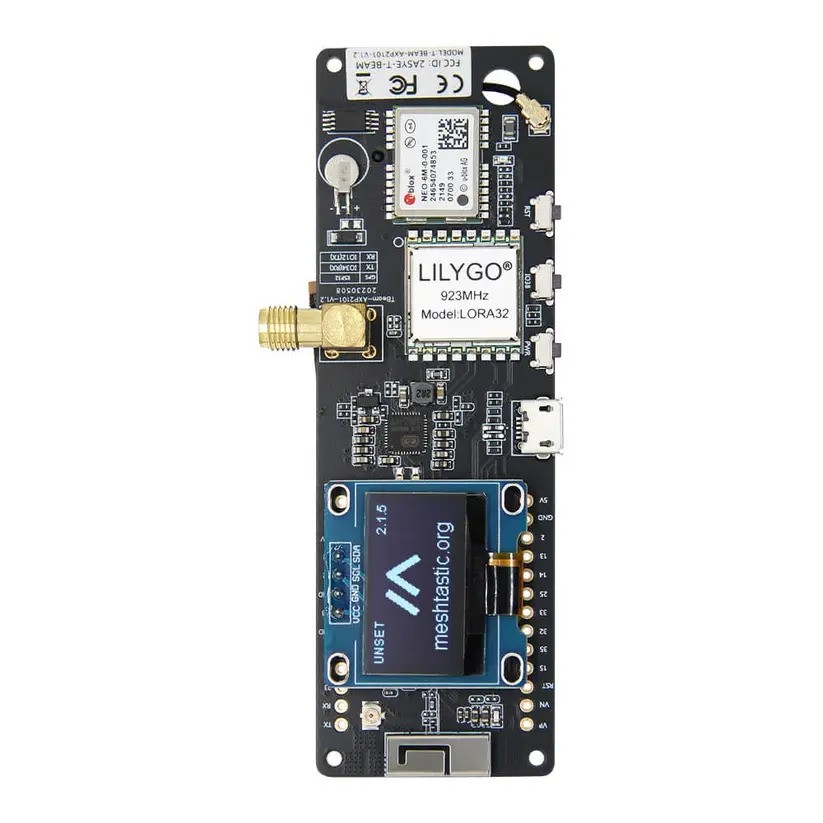
\includegraphics[width=0.8\textwidth]{images/esp32lora.jpg}
    \caption{ESP32 (LilyGo T-Beam) module used in PiIrrigate}
    \label{fig:esp32lora}
\end{figure}

\subsection{Raspberry Pi 4 Model B}
The Raspberry Pi 4 Model B is a small, affordable computer that can be used for a wide range of applications.
It is equipped with a quad-core ARM Cortex-A72 processor, up to 8GB of RAM, and supports dual-band Wi-Fi and Bluetooth.
The Raspberry Pi 4 Model B together with an ESP32LoRa is used in the PiIrrigate project as the gateway that receives data from the ESP32 nodes
and sends it to IoT Hub.
\begin{figure}[H]
    \centering
    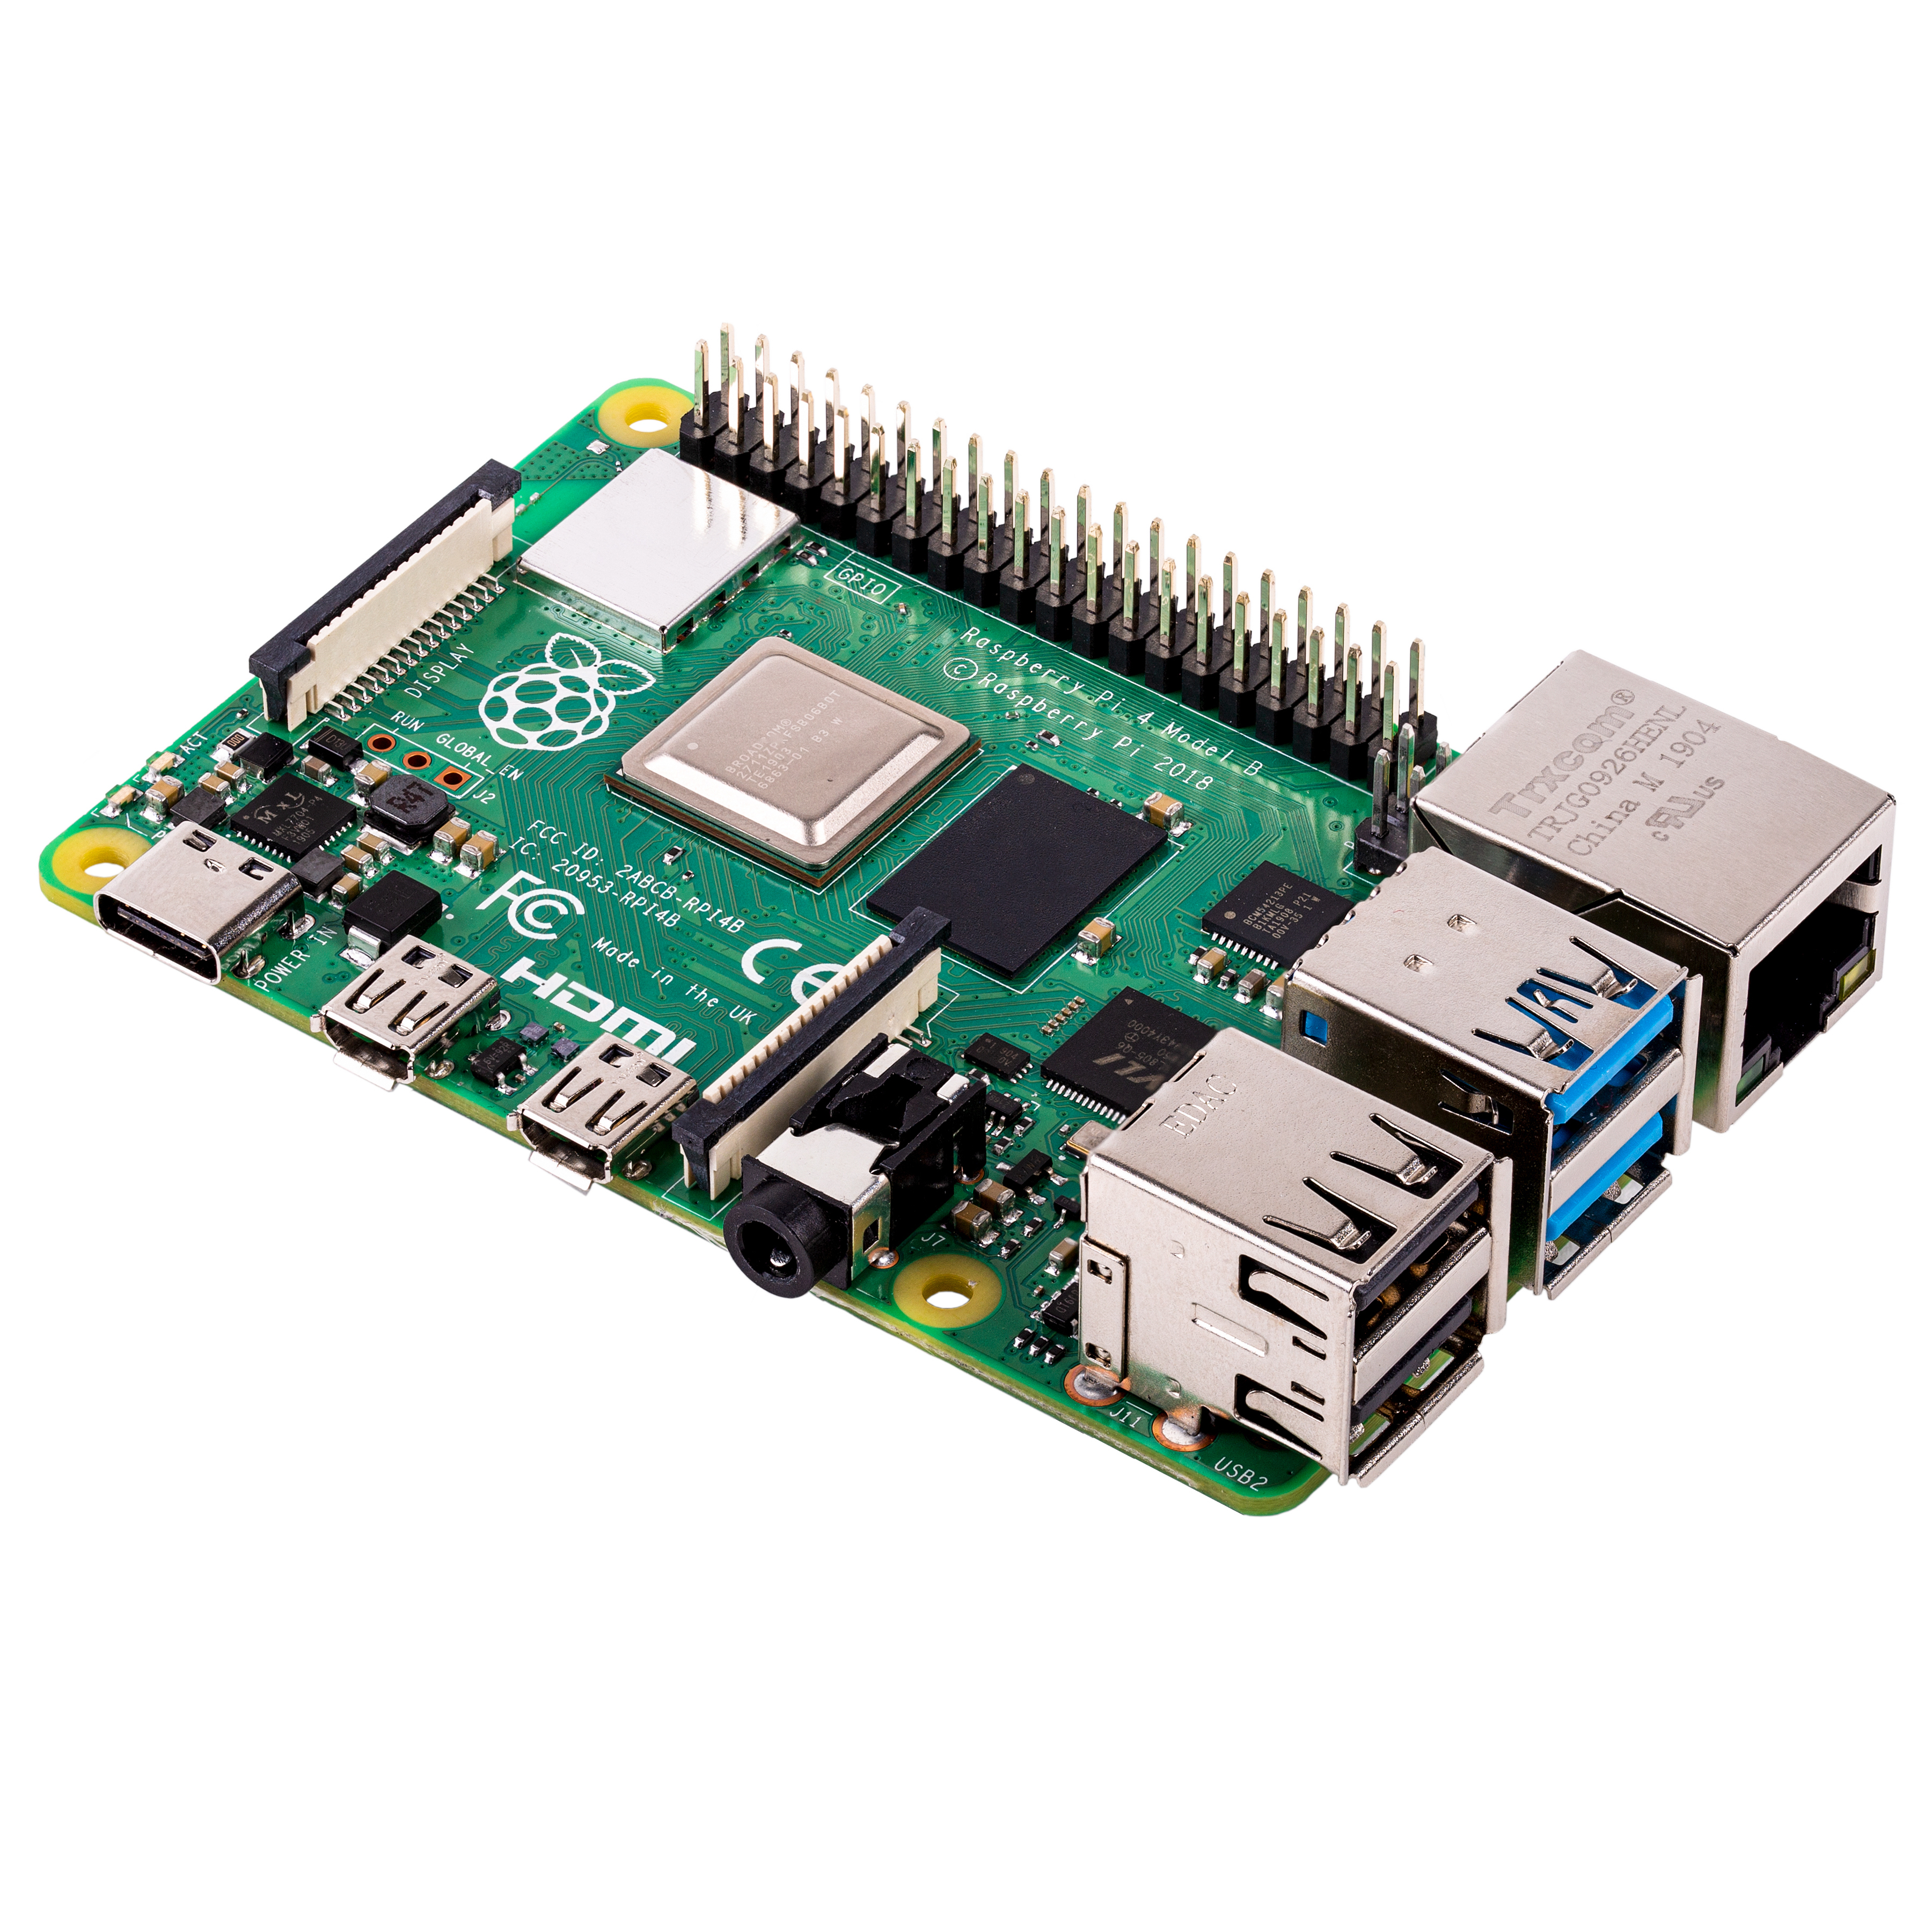
\includegraphics[width=0.8\textwidth]{images/raspberrypi.jpg}
    \caption{Raspberry Pi 4 Model B used in PiIrrigate}
    \label{fig:raspberrypi}
\end{figure}

\section{Data Flow}
The data flow in the PiIrrigate system is as follows:

\begin{enumerate}
  \item The ESP32 nodes collect data from the sensors and send it to the gateway using LoRa radio communication.
  \item The Raspberry Pi receives the data from the ESP32 nodes and sends it to Azure IoT Hub using MQTT protocol.
  \item The web API receives the data from Azure IoT Hub and stores it in the PostgreSQL database using Entity Framework Core. 
  \item The web application retrieves the data from the web API and displays it to the user in real-time using SignalR.
\end{enumerate}
\begin{figure}[H]
    \centering
    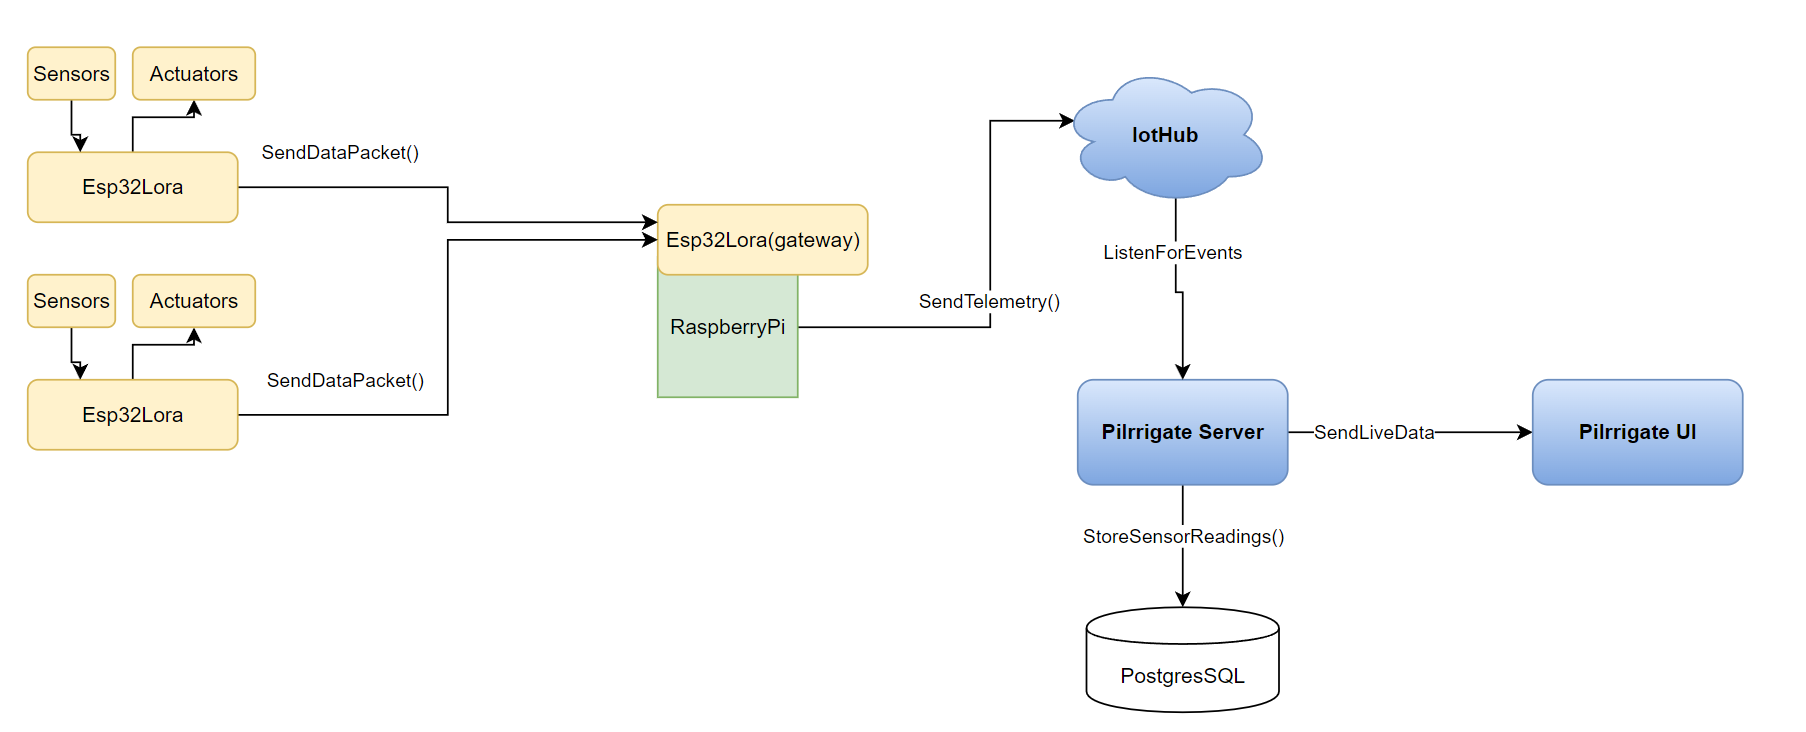
\includegraphics[width=0.8\textwidth]{images/system.png}
    \caption{PiIrrigate System overview}
    \label{fig:system-overview}
\end{figure}

\subsection{Data aquisition}
The data acquisition is done using the ESP32 nodes that collect data from the sensors.
For each sensor type, I created a specific library thath can be used to read the data from the sensor.
Temperature and humidity data is collected using a DHT11 sensor. The communication with the sensor is done using
1-wire digital interface. The communication is done in 3 steps\cite{1wire}:
\begin{enumerate}
  \item The microcontroller initiates communication by sending the start signal.
  The start signal is an 18\,ms LOW signal followed by a $20$--$40\,\mu$s HIGH signal.
  \item The sensor responds a fixed LOW and HIGH handshake pattern, indicating that it is ready to send data.
  Usually the acknowledgment is a $80\,\mu$s LOW signal followed by a $80\,\mu$s HIGH signal.
  \item After the handshake, the sensor sends a 40-bit data stream, which includes the humidity and temperature data.
  The bits are sent in a specific order: first the humidity data (16 bits), 
  then the temperature data (16 bits), 
  and finally a checksum (8 bits).
  Each bit is sent as a $50\,\mu$s LOW signal followed by a HIGH signal that lasts for either $26$--$28\,\mu$s (for a 0 bit) or $70\,\mu$s (for a 1 bit).
  In code, for each bit, the microcontroller waits for the LOW signal to start, 
  then waits for $30\,\mu$s then ig the signal is HIGH, the bit is a 1, otherwise it is a 0.
  The checksum is used to verify the integrity of the data received from the sensor.
\end{enumerate}

\begin{figure}[H]
    \centering
    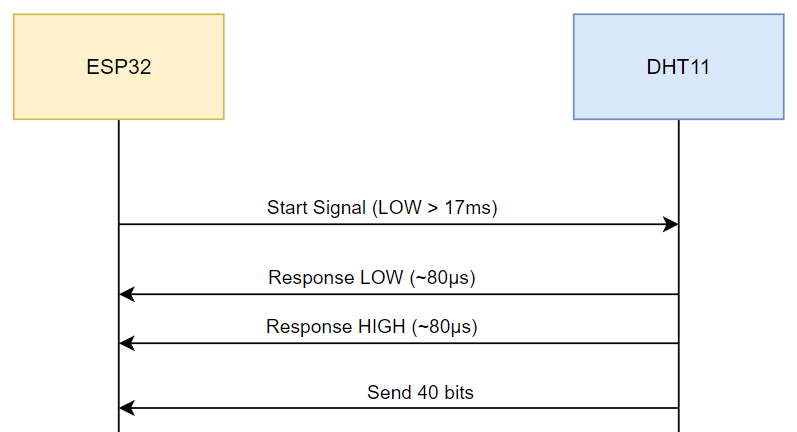
\includegraphics[width=0.8\textwidth]{images/dht-steps.png}
    \caption{Steps in data aquisition from DHT11 sensor}
    \label{fig:dht-steps}
\end{figure}

For the soil moisure data acquisition, I used a resistive soil moisture sensor. The principle of operation is based
on measuring the resistance of the soil. The sensor consists of two probes that are inserted into the soil.
When the soil is dry, the resistance between the probes is high, and when the soil is wet, the resistance is low\cite{s20020363}.
Then an ADC is used to measure the voltage across the probes, which is transofmerd into digital value. In this case, the
ADC is a 12-bit ADC, which means that the digital value can range from 0 to 4095.

For the rain sensor, I used a resistive rians sensor. The principle of operation is similar to the soil moisture sensor,
but it is designed to detect the presence of water on the sensor surface. 
When the sensor is dry, the resistance between the probes is high, and when it is wet, the resistance is low.

\begin{figure}[H]
    \centering
    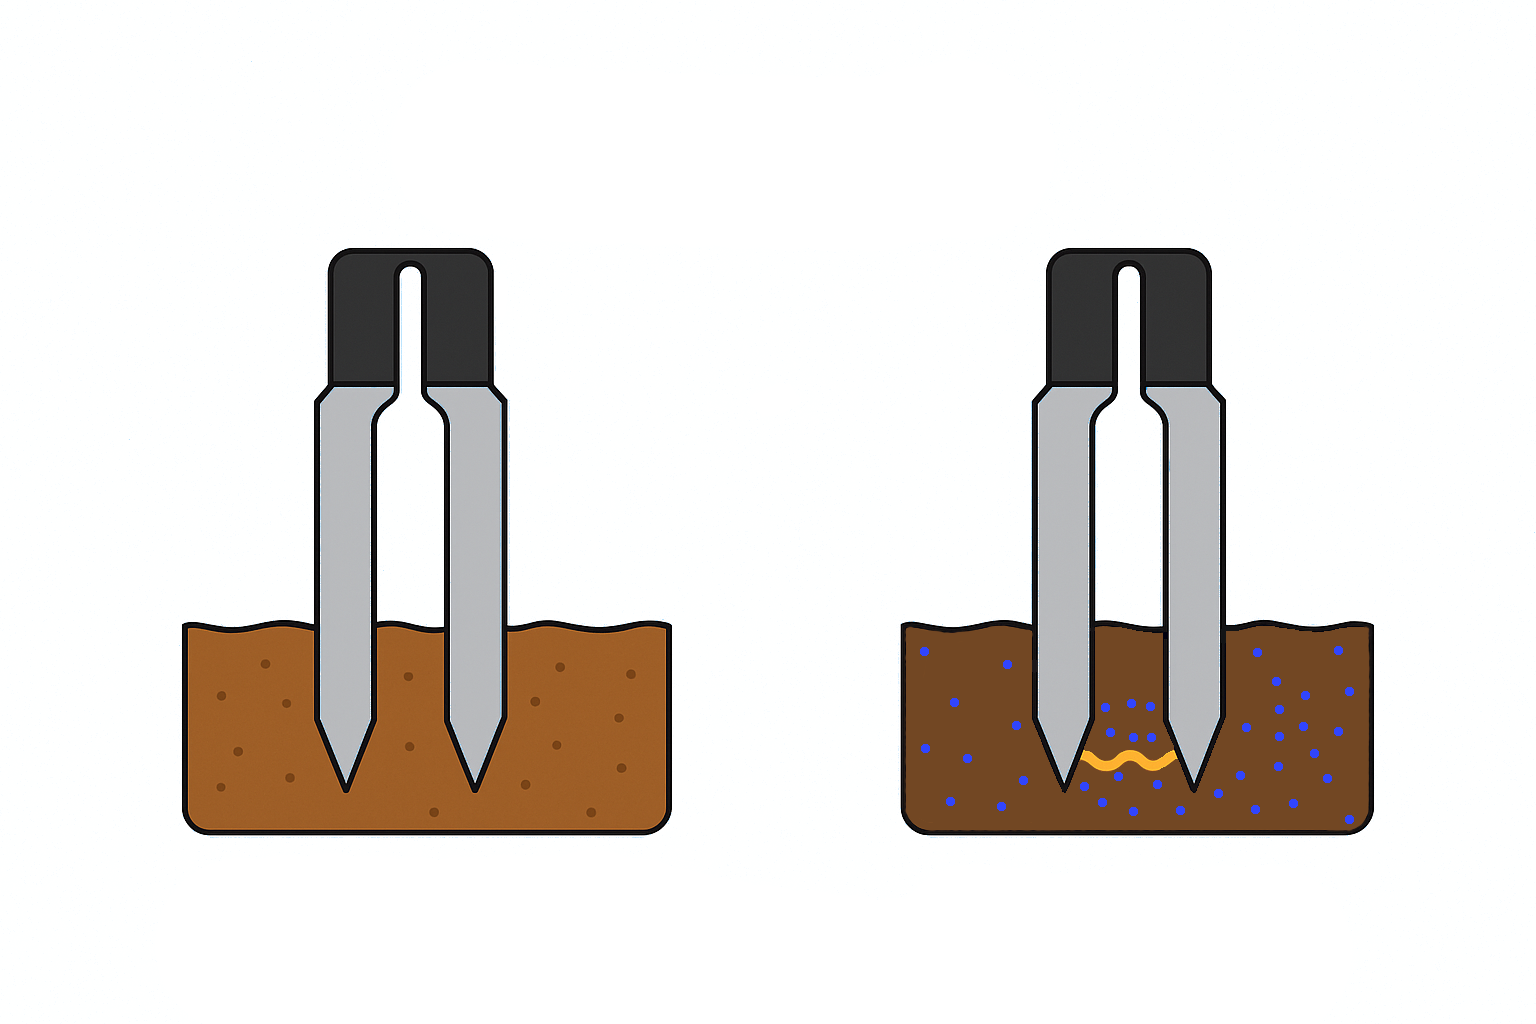
\includegraphics[width=0.7\textwidth]{images/moisture-sensor.png}
    \caption{Soil moisture sensor based on resistive principle}
    \label{fig:moisture-sensor}
\end{figure}

Since the water consumoption is a very important aspect in agriculture, 
I wanted to add a water flow sensor to the system. For the purpose of this project I used an 
YF-S201 water flow sensor, 
which is a low-cost sensor that can be used to measure the flow rate of water in a pipe.
The sensor consists of a plastic body with a 
turbine inside that rotates when water flows through it.
The rotation of the turbine generates a pulse signal that can be used to measure the 
flow rate of water.
The sensor has a maximum flow rate of 30 liters per minute and a minimum 
flow rate of 1 liter per minute.
The sensor has three wires: red (VCC), black (GND), and yellow (signal).
At each rotation of the tubine, the sesnsor generates a pulse signal on the signal wire.
The ESP32 counts the number of pulses in a given time interval 
(e.g., 1 second) to calculate the flow rate.
The flow rate can be calculated using the following formula:
\begin{equation}
    \text{Flow Rate} = \frac{\text{Number of Pulses} \times 60}{\text{Time Interval (seconds)}}
\end{equation}
\begin{figure}[H]
    \centering
    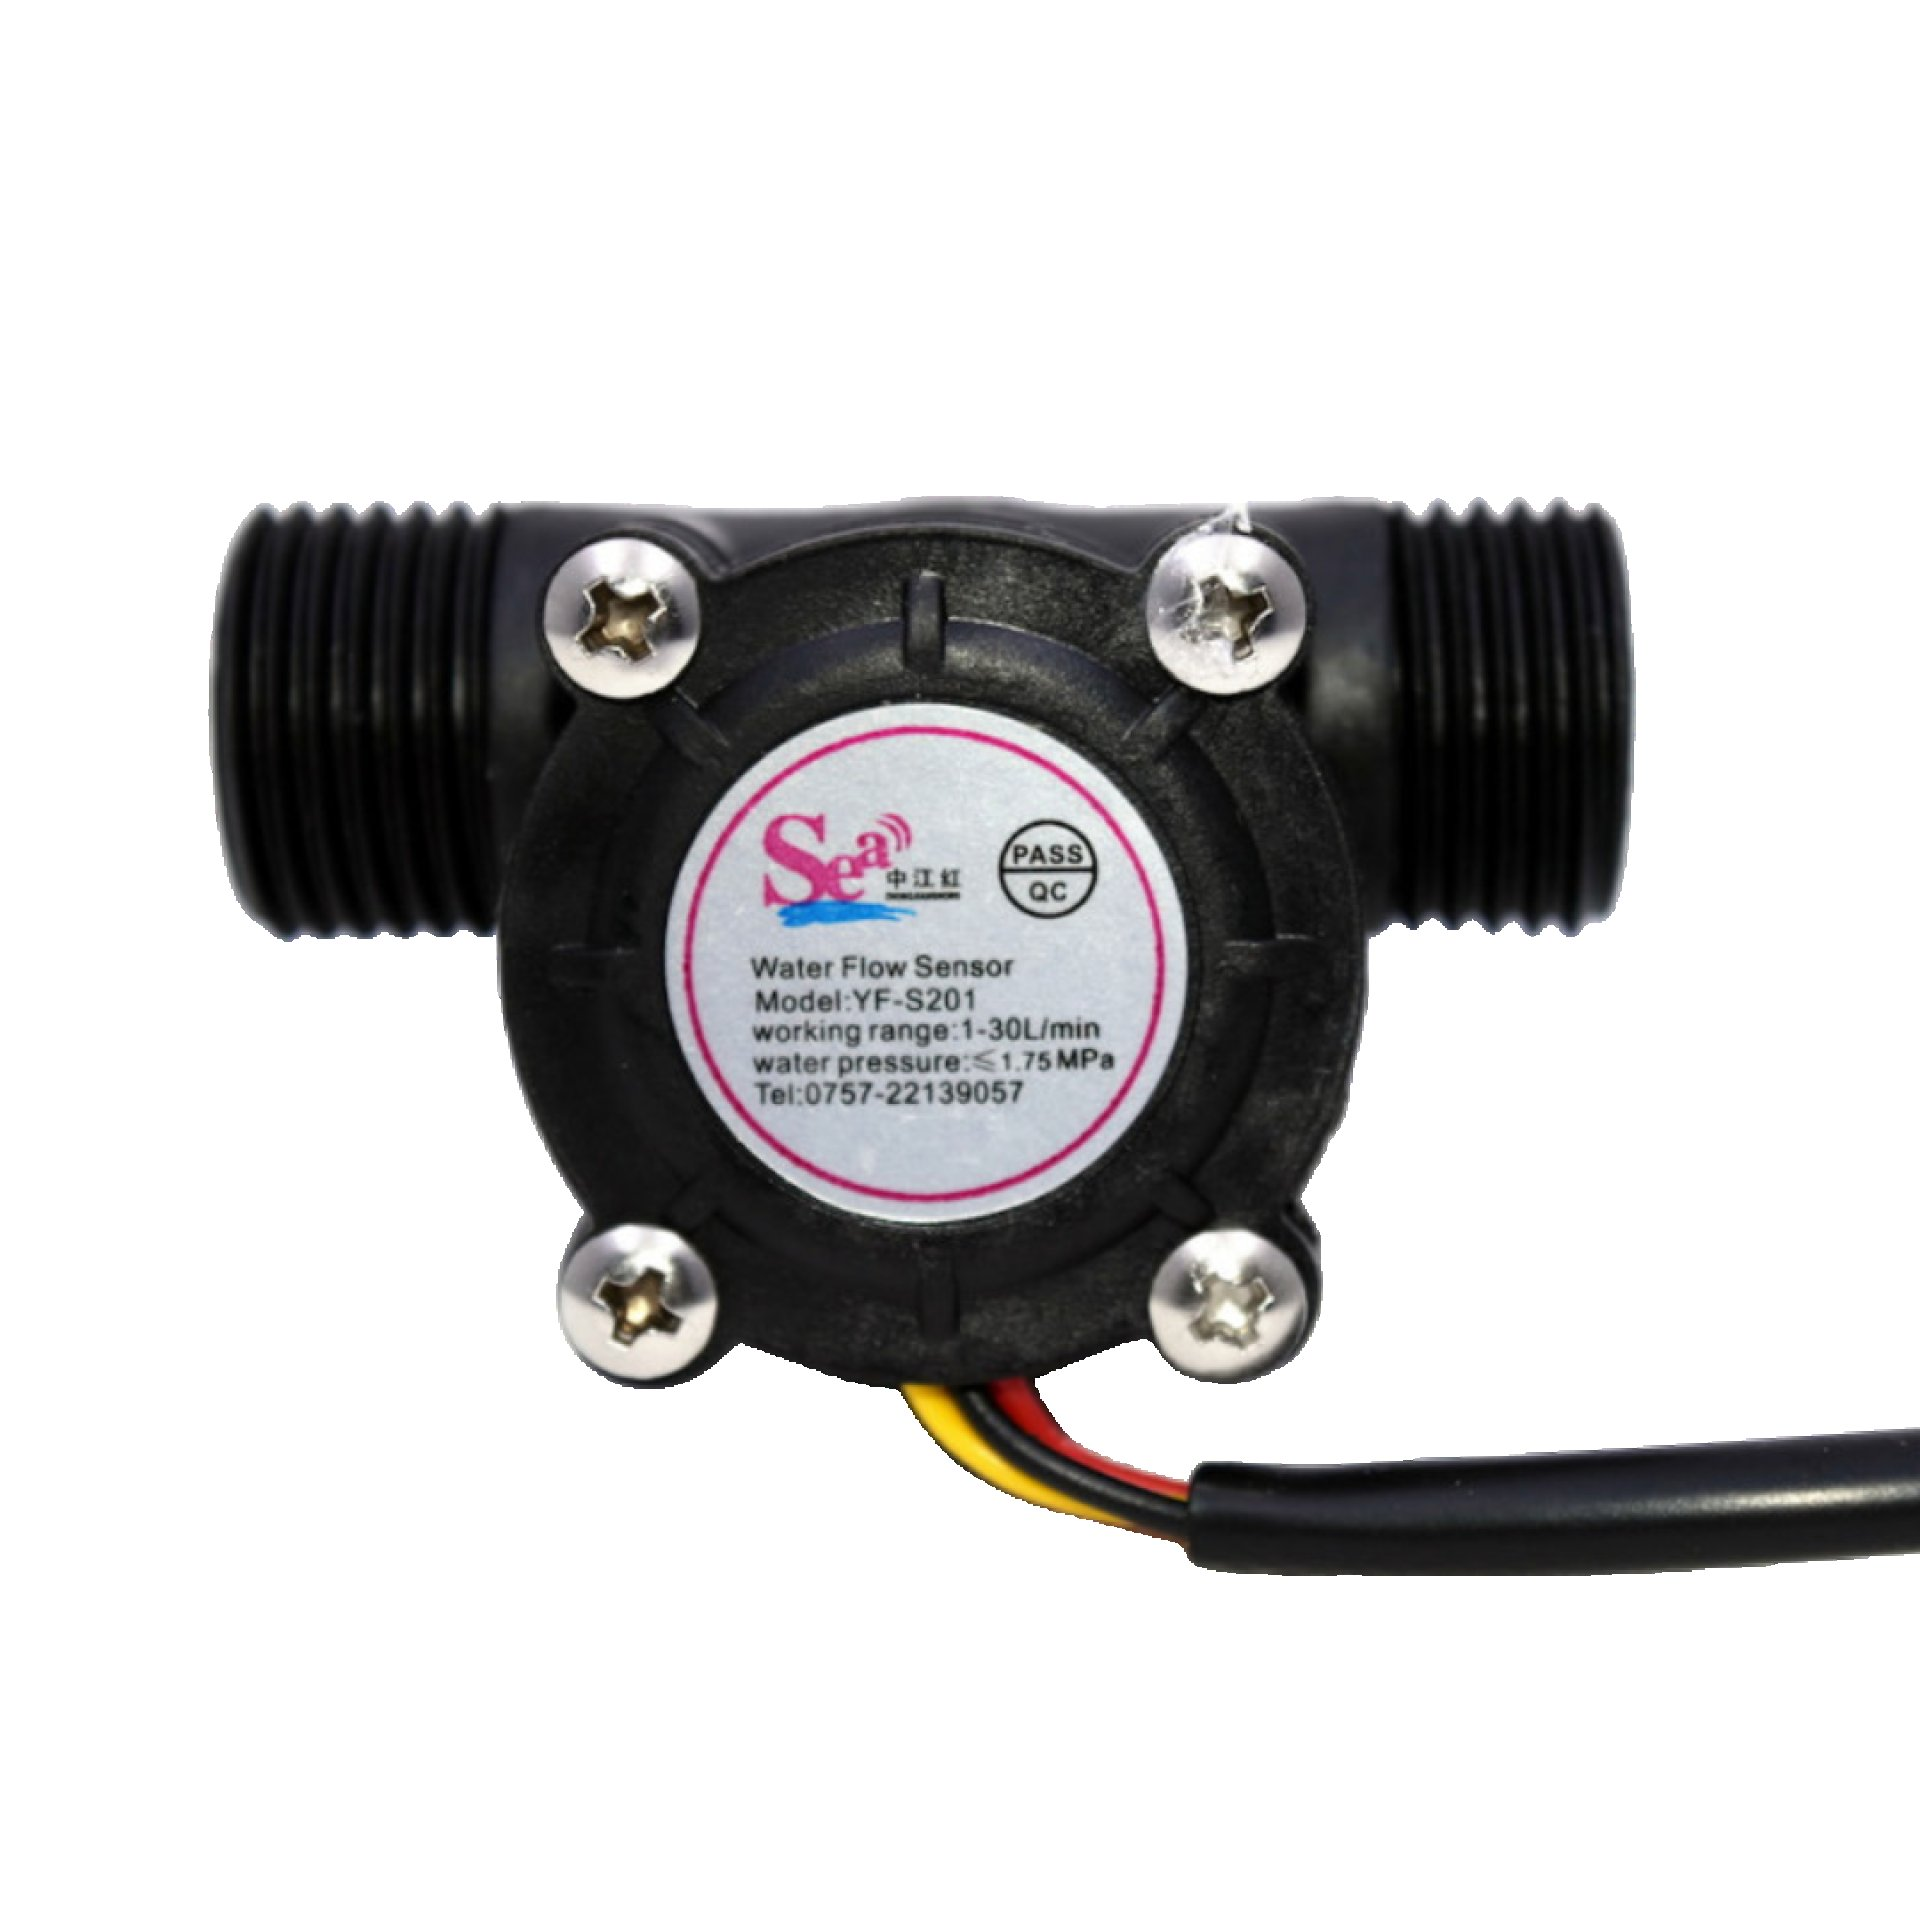
\includegraphics[width=0.5\textwidth]{images/water-flow.jpg}
    \caption{Water flow sensor used in PiIrrigate}
    \label{fig:water-flow-sensor}
\end{figure}

In my implementation, the water will be in a container, and during the irrigation process, 
the water will be deliverd to the plants using the gravity force. Because of this, I used
water temperature sensor to measure the temperature of the water in the container. 
The water temperature sensor is a DS18B20 sensor, 
which is a digital temperature sensor that can be used to measure the temperature of liquids.
The DS18B20 sensor uses the 1-wire digital interface to communicate with the ESP32.
The sensor can measure temperatures from -55°C to +125°C with an accuracy of ±0.5°C.

\begin{figure}[H]
    \centering
    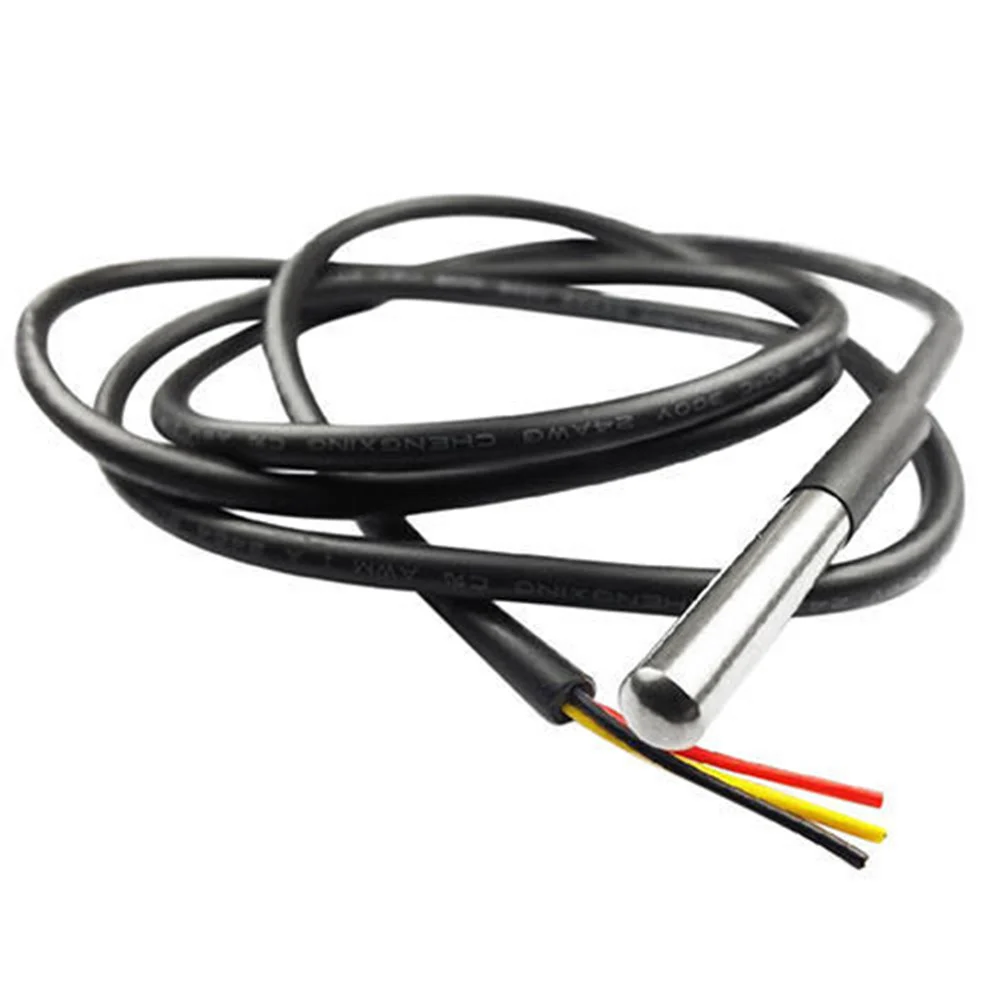
\includegraphics[width=0.5\textwidth]{images/water-temp.png}
    \caption{DS18B20 water temperature sensor used in PiIrrigate}
    \label{fig:ds18b20}
\end{figure}

Beside the sensors, I also used the GPS module of the T-Beam ESP32 board to 
ollect the GPS coordinates of the node. 
This can be useful for tracking the location of the node and for mapping the irrigation system.

\subsection{ESP32 Pinout and Sensor Connections}
The ESP32 board has a variety of pins that can be used to connect the sensors and other components.
In the following diagram the connecttions between the ESP32 board and the sensors are shown.
\begin{figure}[H]
    \centering
    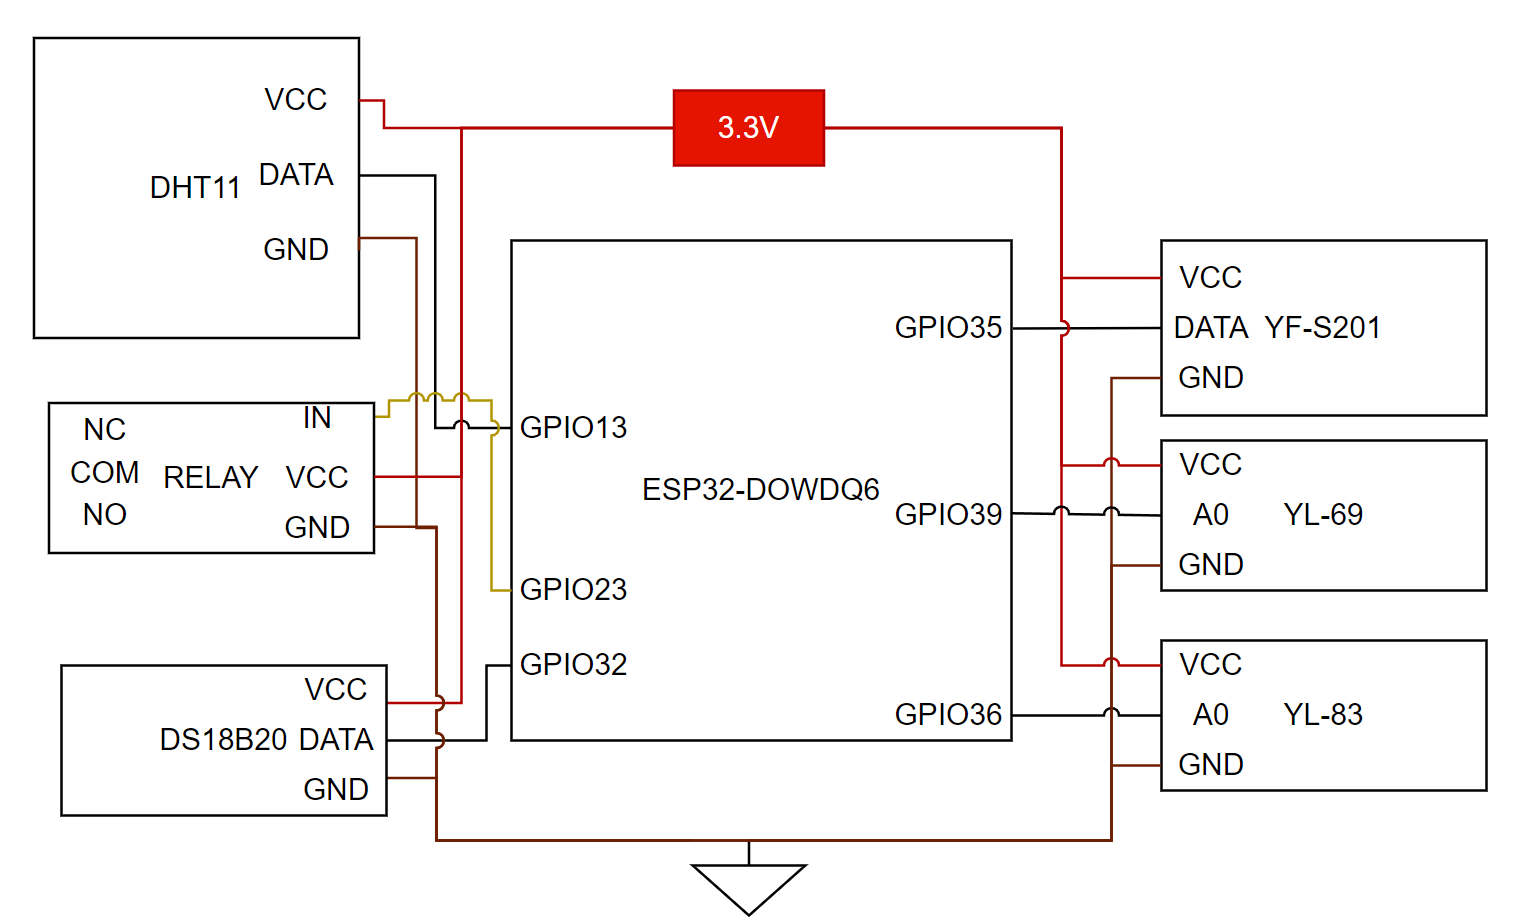
\includegraphics[width=0.8\textwidth]{images/esp-diagram.png}
    \caption{ESP32 pinout and connections}
    \label{fig:esp32-pinout}
\end{figure}

\subsection{ESP32 LoRa Communication}
As I mentioned before, the communication between the ESP32 nodes and the gateway is done using
LoRa radio communication. For this purpose, I used te Lora library for Arduino, which is a 
popular library for LoRa communication. 
I chose to use the LoRa library because it is easy to use and it makkes the PiIrrigate system more
robust and reliable since the library handles the low-level details of the LoRa communication.

Every 10 seconds, the data is collected from the sensors and sent to the gateway in the form of packets.
Each packet contains the following data:
\begin{itemize}
  \item \textbf{C:} Packet count - a counter that is incremented for each packet sent.
  \item \textbf{ID:} Board MAC address - a unique identifier for the ESP32 node.
  \item \textbf{T:} Temperature - the temperature measured by the DHT11 sensor.
  \item \textbf{H:} Humidity - the humidity measured by the DHT11 sensor.
  \item \textbf{S:} Soil moisture - the soil moisture measured by the soil moisture sensor.
  \item \textbf{R:} Rain - the rain sensor value, which is either 0 (no rain) or 1 (rain detected).
  \item \textbf{WT:} Water temperature - the water temperature measured by the DS18B20 sensor.
  \item \textbf{WF:} Water flow - the water flow measured by the water flow sensor.
  \item \textbf{GPS:} GPS coordinates - the latitude and longitude of the node, obtained from the GPS module.
\end{itemize}

Each time a packet is sent, the ESP32 node waits for an acknowledgment from the gateway. 
If the acknowledgment is received, the packet is considered sent successfully.
If the acknowledgment is not received, the ESP32 node will retry sending the packet up to 3 times. 
After 3 retries, the packet is considered lost and the ESP32 node will log an error message.
If the packet reaches the gateway, the gateway will send the packet to the Raspberry Pi via UART.
